% Standalone TikZ figure for proposed candidate screening and validation.
% Compile with pdfLaTeX. Attention cell is an illustrative architecture choice.
\documentclass[11pt]{article}
\usepackage[paperwidth=29cm,paperheight=20cm,margin=5mm]{geometry}
\usepackage[T1]{fontenc}
\usepackage{lmodern,amsmath,amssymb,tikz}
\usetikzlibrary{arrows.meta,calc}
\pagestyle{empty}
\definecolor{outline}{HTML}{153543}
\definecolor{norm}{HTML}{B9CDD0}
\definecolor{attn}{HTML}{ECE6D8}
\definecolor{ffn}{HTML}{B9B2C4}
\definecolor{linear}{HTML}{D8B5BE}
\definecolor{comp}{HTML}{A8D5CE}
\definecolor{analog}{HTML}{C9BEDA}
\begin{document}
\noindent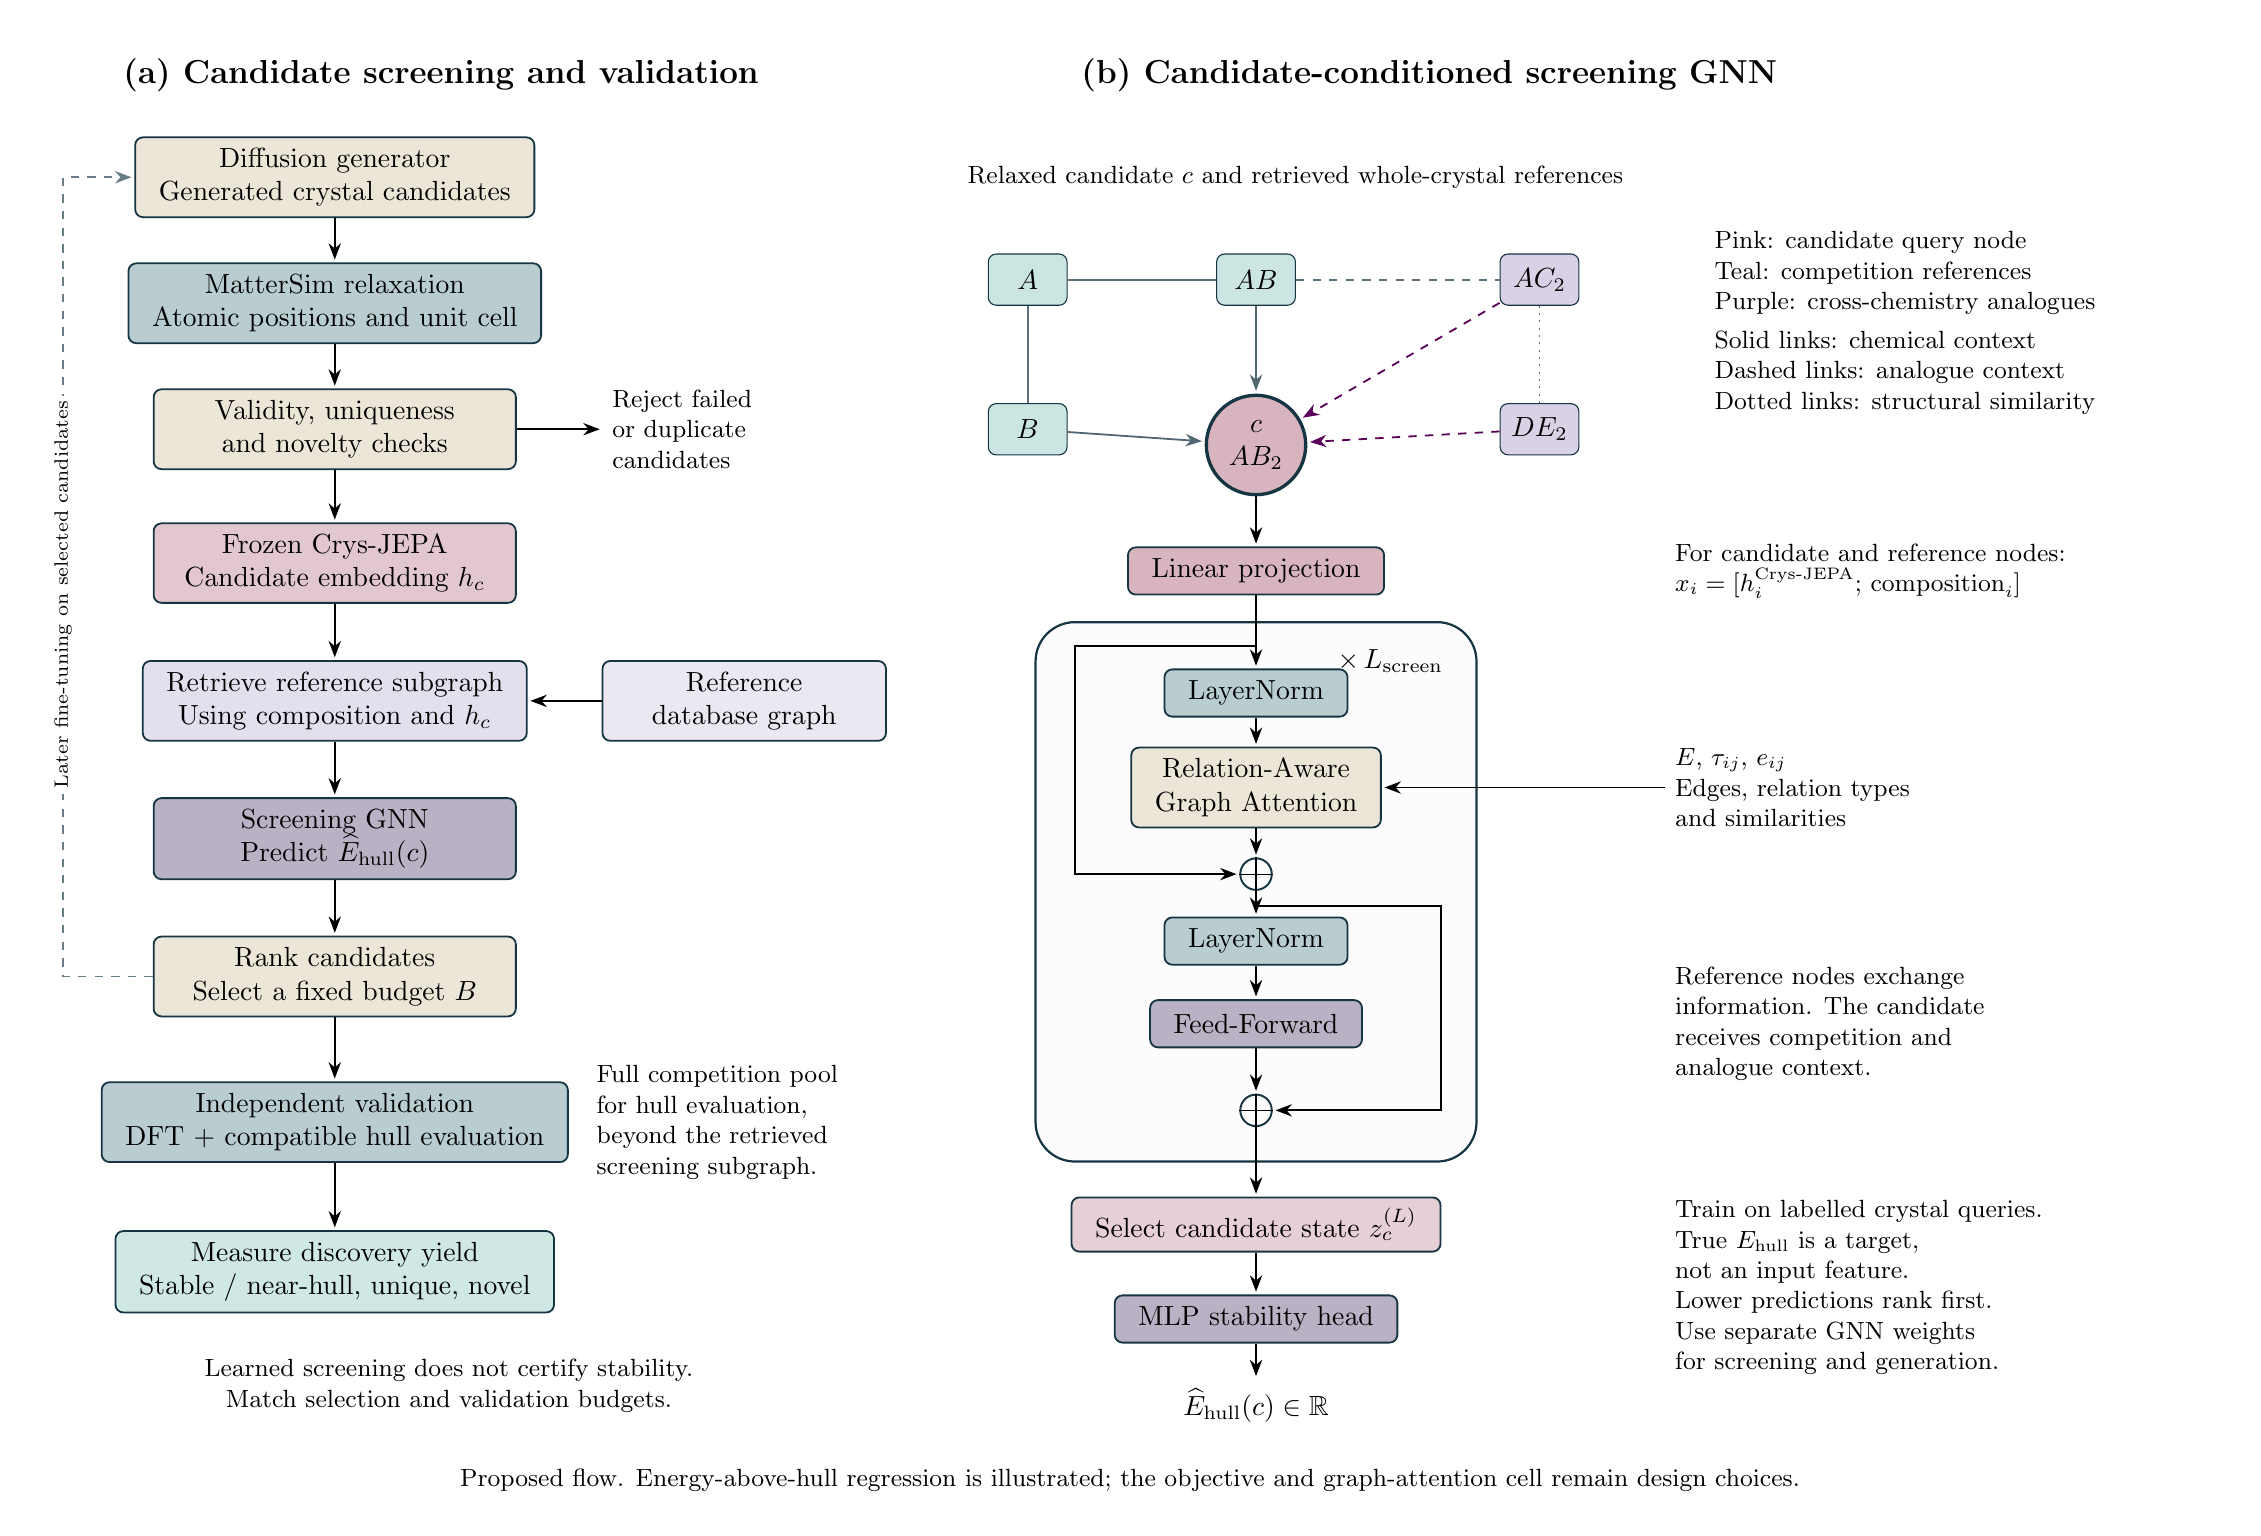
\begin{tikzpicture}[x=1cm,y=1cm,>=Stealth,
 layer/.style={draw=outline,line width=.65pt,rounded corners=1mm,align=center,minimum height=.6cm,inner xsep=3mm,inner ysep=1.4mm},
 arrow/.style={->,line width=.65pt,shorten >=1pt},
 add/.style={circle,draw=outline,line width=.7pt,minimum size=4mm,inner sep=0pt},
 ref/.style={draw=outline,fill=comp!60,rounded corners=1mm,minimum width=1.0cm,minimum height=.65cm},
 edge/.style={draw=outline!70,line width=.65pt}]
\path[use as bounding box] (0,0) rectangle (28,18.8);
\node[font=\large\bfseries] at (5.25,18.2) {(a) Candidate screening and validation};
\node[font=\large\bfseries] at (17.8,18.2) {(b) Candidate-conditioned screening GNN};

% Part a. Read from top to bottom.
\node[layer,fill=attn,minimum width=4.6cm] (gen) at (3.9,16.9) {Diffusion generator\\Generated crystal candidates};
\node[layer,fill=norm,minimum width=4.6cm] (relax) at (3.9,15.3) {MatterSim relaxation\\Atomic positions and unit cell};
\node[layer,fill=attn,minimum width=4.6cm] (filter) at (3.9,13.7) {Validity, uniqueness\\and novelty checks};
\node[layer,fill=linear!75,minimum width=4.6cm] (embed) at (3.9,12.0) {Frozen Crys-JEPA\\Candidate embedding $h_c$};
\node[layer,fill=analog!50,minimum width=4.6cm] (retrieve) at (3.9,10.25) {Retrieve reference subgraph\\Using composition and $h_c$};
\node[layer,fill=ffn,minimum width=4.6cm] (screen) at (3.9,8.5) {Screening GNN\\Predict $\widehat E_{\mathrm{hull}}(c)$};
\node[layer,fill=attn,minimum width=4.6cm] (rank) at (3.9,6.75) {Rank candidates\\Select a fixed budget $B$};
\node[layer,fill=norm,minimum width=4.6cm] (dft) at (3.9,4.9) {Independent validation\\DFT + compatible hull evaluation};
\node[layer,fill=comp!55,minimum width=4.6cm] (yield) at (3.9,3.0) {Measure discovery yield\\Stable / near-hull, unique, novel};
\foreach \a/\b in {gen/relax,relax/filter,filter/embed,embed/retrieve,retrieve/screen,screen/rank,rank/dft,dft/yield}
 \draw[arrow] (\a)--(\b);
\node[align=left,font=\small,text width=2.3cm,anchor=west] (reject) at (7.3,13.7) {Reject failed\\or duplicate\\candidates};
\draw[arrow] (filter.east)--(reject.west);
\node[layer,fill=analog!35,text width=3.0cm] (db) at (9.1,10.25) {Reference\\database graph};
\draw[arrow] (db.west)--(retrieve.east);
\node[align=left,font=\small,anchor=west] at (7.1,4.9) {Full competition pool\\for hull evaluation,\\beyond the retrieved\\screening subgraph.};
\node[align=center,font=\small] at (5.35,1.55)
 {Learned screening does not certify stability.\\Match selection and validation budgets.};

% Part b. Retrieved references plus the completed candidate as query node.
\node[font=\small,align=center] at (16.1,16.9) {Relaxed candidate $c$ and retrieved whole-crystal references};
\node[ref] (a) at (12.7,15.6) {$A$};
\node[ref] (ab) at (15.6,15.6) {$AB$};
\node[ref,fill=analog!70] (ac) at (19.2,15.6) {$AC_2$};
\node[ref] (b) at (12.7,13.7) {$B$};
\node[ref,fill=analog!70] (de) at (19.2,13.7) {$DE_2$};
\node[draw=outline,fill=linear,very thick,circle,minimum size=1.2cm,align=center] (cand) at (15.6,13.5) {$c$\\$AB_2$};
\draw[edge] (a)--(ab);
\draw[edge] (a)--(b);
\draw[edge,dashed] (ab)--(ac);
\draw[edge,dotted] (ac)--(de);
\draw[arrow,draw=outline!75] (ab)--(cand);
\draw[arrow,draw=outline!75] (b)--(cand);
\draw[arrow,dashed,draw=violet!70!black] (ac)--(cand);
\draw[arrow,dashed,draw=violet!70!black] (de)--(cand);
\node[align=left,font=\small,anchor=west] at (21.3,15.05)
 {Pink: candidate query node\\Teal: competition references\\Purple: cross-chemistry analogues\\[3pt]Solid links: chemical context\\Dashed links: analogue context\\Dotted links: structural similarity};

% Downward pre-norm graph cell. Every node is updated; read out the candidate only.
\node[layer,fill=linear,minimum width=3.2cm] (proj) at (15.6,11.9) {Linear projection};
\draw[arrow] (cand)--(proj);
\node[align=left,font=\small,text width=5.7cm,anchor=west] at (20.8,11.9)
 {For candidate and reference nodes:\\$x_i=[h_i^{\mathrm{Crys\text{-}JEPA}};\,\mathrm{composition}_i]$};
\draw[draw=outline,rounded corners=5mm,line width=.8pt,fill=black!1]
 (12.8,4.4) rectangle (18.4,11.25);
\node[anchor=north east] at (18.1,11.03) {$\times\,L_{\mathrm{screen}}$};
\node[layer,fill=norm] (ln1) at (15.6,10.35) {LayerNorm};
\node[layer,fill=attn,minimum width=3.0cm,minimum height=.85cm] (gat) at (15.6,9.15) {Relation-Aware\\Graph Attention};
\node[add] (sum1) at (15.6,8.05) {};
\node[layer,fill=norm] (ln2) at (15.6,7.2) {LayerNorm};
\node[layer,fill=ffn,minimum width=2.65cm] (ff) at (15.6,6.15) {Feed-Forward};
\node[add] (sum2) at (15.6,5.05) {};
\foreach \s in {sum1,sum2}{\draw (\s.west)--(\s.east) (\s.south)--(\s.north);}
\foreach \a/\b in {proj/ln1,ln1/gat,gat/sum1,sum1/ln2,ln2/ff,ff/sum2}
 \draw[arrow] (\a)--(\b);
\draw[arrow] (15.6,10.95)--(13.3,10.95)|-(sum1.west);
\draw[arrow] (15.6,7.65)--(17.95,7.65)|-(sum2.east);
\node[align=left,font=\small,anchor=west] (edges) at (20.8,9.15)
 {$E,\,\tau_{ij},\,e_{ij}$\\Edges, relation types\\and similarities};
\draw[arrow] (edges.west)--(gat.east);
\node[align=left,font=\small,anchor=west] at (20.8,6.15)
 {Reference nodes exchange\\information. The candidate\\receives competition and\\analogue context.};
\node[layer,fill=linear!65,minimum width=3.2cm] (readout) at (15.6,3.6) {Select candidate state $z_c^{(L)}$};
\node[layer,fill=ffn,minimum width=3.2cm] (head) at (15.6,2.4) {MLP stability head};
\node (score) at (15.6,1.3) {$\widehat E_{\mathrm{hull}}(c)\in\mathbb R$};
\draw[arrow] (sum2)--(readout);
\draw[arrow] (readout)--(head);
\draw[arrow] (head)--(score);
\node[align=left,font=\small,anchor=west] at (20.8,2.8)
 {Train on labelled crystal queries.\\True $E_{\mathrm{hull}}$ is a target,\\not an input feature.\\Lower predictions rank first.\\Use separate GNN weights\\for screening and generation.};
% Selection can supply a later training round; inference does not update weights.
\draw[arrow,dashed,draw=outline!65] (rank.west)--(.45,6.75)--(.45,16.9)--(gen.west);
\node[rotate=90,font=\scriptsize,fill=white,inner sep=2pt] at (.45,11.6)
 {Later fine-tuning on selected candidates};
\node[align=center,font=\small] at (14,.35)
 {Proposed flow. Energy-above-hull regression is illustrated; the objective and graph-attention cell remain design choices.};
\end{tikzpicture}
\end{document}
